\documentclass{standalone}
\usepackage{tikz}
\usetikzlibrary{shapes.geometric}
\begin{document}
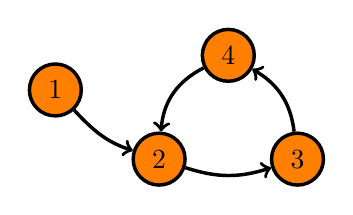
\begin{tikzpicture}
[every node/.style={inner sep=0pt}]
\node (1) [circle, minimum size=18.75pt, fill=orange, line width=1.25pt, draw=black] at (37.5pt, -37.5pt) {\textcolor{black}{1}};
\node (2) [circle, minimum size=18.75pt, fill=orange, line width=1.25pt, draw=black] at (75.0pt, -62.5pt) {\textcolor{black}{2}};
\node (3) [circle, minimum size=18.75pt, fill=orange, line width=1.25pt, draw=black] at (125.0pt, -62.5pt) {\textcolor{black}{3}};
\node (4) [circle, minimum size=18.75pt, fill=orange, line width=1.25pt, draw=black] at (100.0pt, -25.0pt) {\textcolor{black}{4}};
\draw [line width=1.25, ->, color=black] (1) to  [in=162, out=313] (2);
\draw [line width=1.25, ->, color=black] (2) to  [in=198, out=342] (3);
\draw [line width=1.25, ->, color=black] (3) to  [in=330, out=97] (4);
\draw [line width=1.25, ->, color=black] (4) to  [in=86, out=207] (2);
\end{tikzpicture}

\end{document}
